\chapter*{Ещё игры}
\addcontentsline{toc}{chapter}{Ещё игры}
%“Half this game is 90\% mental.”
%-- Danny Ozark manager of the Phillies baseball team.

\setlength{\epigraphwidth}{.6\textwidth}
\epigraph{Половина этой игры на 90\% идёт в уме.}{---Дэнни Озарк, тренер Филадельфийской бейсбольной команды.}

Вообще говоря, анализ игры часто требует решения двух задач: нахождения правильной стратегии и нахождения убедительного аргумента, который показывает, что стратегия наилучшая из возможных.
(Такой аргумент может быть правильной стратегией для другого игрока.)

Но, иногда можно отделаться довольно легко.
Рассмотрим следующую невинную с виду задачу.

\subsection*{Щёлк}% (CHOMP)
\rindex{Щёлк}

Два игрока по очереди откусывают от прямоугольной шоколадки, сотоящей из $m \times n$ квадратных долек.
Каждый раз игрок выбирает дольку и откусывает её вместе со всеми дольками находящимися сверху и справа от неё.
Каждый игрок старается избежать левую нижнюю дольку, которая отравлена.

Докажите, что если шоколадка состоит больше, чем из одной дольки, то у первого игрока есть выигрышная стратегия.

\begin{figure}[h!]
\centering
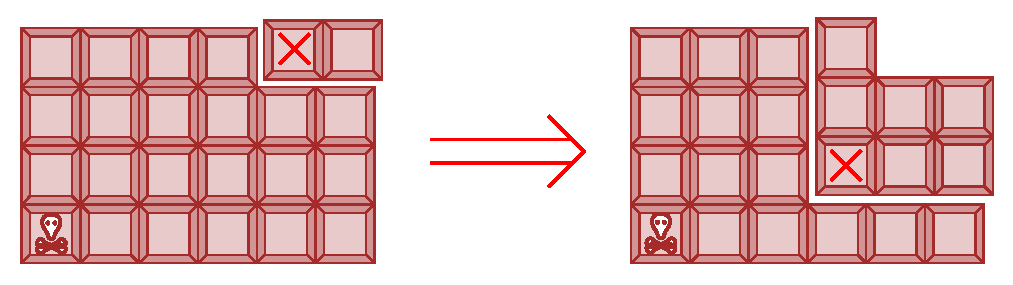
\includegraphics[scale=0.5]{Figs/MoreGames/chomp}
\end{figure}

\paragraph{Решение:} Либо у первого игрока (Алисы), либо у второго (Боба) должна быть выигрышная стратегия.
Предположим, она у Боба.
Тогда, в частности, у Боба должен быть выигрышный ответ на первый ход Алисы, когда она просто откусывает верхнюю дольку справа.

Но какой бы ни был ответ Боба, Алиса может сделать таким же свой первый ход, что противоречит предположению о том, что Боб всегда может выиграть.
Отсюда следует,
что выигрышная стратегия должна быть у Алисы.
\heart

Такой вид доказательства известен как \emph{заимствование стратегии} и он, к сожалению, ничего не говорит нам о том, как же, собственно, Алисе выигрывать игру.
В последней главе подробнее рассказывается об игре «Щёлк», её истории и более общей версии.

\medskip

Для решения оставшихся задач-игр используются разнообразные методы.

\subsection*{Детерминированный покер}% (DETERMENISTIC POKER)
\rindex{Детерминированный покер}

Не желая зависеть от капризного случая, Алиса и Боб решили сыграть в абсолютно детерминированную версию пятикарточного покера (так называемый дро-покер).
Колода карт раскладывается на столе в открытую.
Алиса выбирает 5 карт, затем Боб берёт 5 карт.
Алиса меняет любое число карт, заменённые карты выходят из игры, то же проделывает и Боб.
Все действия производятся в открытую на виду у оппонента.
Игрок с лучшей комбинацией выигрывает.
Поскольку Алиса ходит первая, то, если конечные комбинации оказываются равносильными, Боб объявляется победителем.
Кто победит при оптимальной игре?

\medskip

Детерминированный покер --- это игра с полной информацией.
В играх, содержащих скрытую информацию или одновременные ходы, может потребоваться вероятностная стратегия.
Говорят, что набор таких стратегий (один для каждого игрока) находится в \emph{равновесии}, если никто из игроков не может увеличить выигрыш, изменив свою стратегию, при условии, что остальные участники своих стратегий не меняют.
Например, в игре «Камень, ножницы, бумага» в (единственной) равновесной стратегии, каждый игрок выбирает все три возможных варианта с одинаковой вероятностью.

\subsection*{Шведская лотерея}% (SWEDISH LOTTERY)
\rindex{Шведская лотерея}

Для Шведской национальной лотереи предлагался следующий механизм игры: каждый участник выбирает целое положительное число.
Объявляется победителем тот, кто называет наименьшее число, никем другим не выбранное.
(Если нет числа, выбранного только одним участником, то победителя нет.)

Если в игре участвуют только три человека, и каждый применяет оптимальную, равновесную, вероятностную стратегию, чему равно наибольшее положительное число, имеющее положительную вероятность быть выбранным?

\subsection*{Блины}% (PANCAKES)
\rindex{Блины}

Алиса и Боб опять проголодались, и перед ними лежат две стопки блинов, высотой в $m$ и $n$ блинов.
Каждый игрок по очереди должен съесть из большей стопки число блинов (ненулевое), кратное количеству блинов в меньшей стопке.
Разумеется, последний блин в каждой стопке непропечённый, так что игрок, который первым заканчивает стопку, проигрывает.

Для какой пары $(m,n)$ у Алисы (она ходит первая) имеется выигрышная стратегия?

Что случается, если у игры обратная цель, то есть побеждает тот, кто первый закончит стопку?

\subsection*{Определение разности}% (DETERMINING A DIFFERENCE)
\rindex{Определение разности}

После завтрака Алиса и Боб решают отдохнуть и сыграть в простую числовую игру.

\medskip

Алиса выбирает цифру и Боб подставляет её вместо звёздочки в выражение «$**** - ****$»; процедура повторяется пока остаются звёздочки. 
Алиса пытается сделать окончательную разность максимальной, a Боб --- минимальной.
Какая разность получится при оптимальной игре?

\subsection*{Тройная дуэль}% (THREE-WAY DUEL)
\rindex{Тройная дуэль}

Алиса, Боб и Кэрол устраивают тройную дуэль.
Алиса --- плохой стрелок, попадает в цель, в среднем, только в $\tfrac13$ случаев.
Боб лучше, попадает в цель с вероятностью $\tfrac23$.
Кэрол --- меткий стрелок, бьёт без промаха.

Они стреляют по очереди, первой Алиса, вторым Боб и третьей Кэрол, затем опять Алиса, и так далее, пока не останется только один стрелок.
Каков для Алисы наилучший план действий?
